% +arr: add circles to nodes

\documentclass[tikz, margin=3mm]{standalone}
    \usetikzlibrary{positioning, shapes.symbols}

\begin{document}
   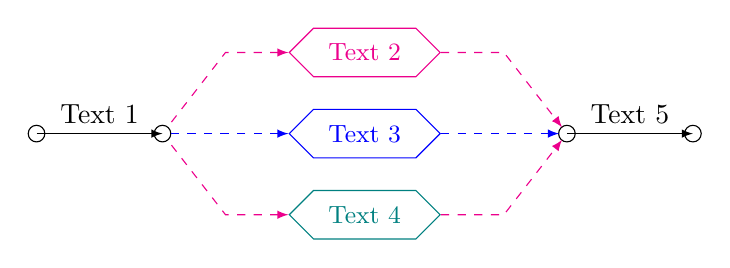
\begin{tikzpicture}[ 
   node distance = 4mm and 16mm,
   mynode/.style = {shape=signal, signal to=west and east,
			                 draw, color = #1,
			                 text width=1.3cm, align=flush center, 
			                 inner xsep=0mm, inner ysep=2mm, font=\small}
                 ]
	% main nodes
	\node (A) [mynode=magenta]            {Text 2};
	\node (B) [mynode=blue, below=of A]   {Text 3};
	\node (C) [mynode=teal, below=of B]   {Text 4};
	
	% coordinates for lines
	\coordinate[left=of B.west]     (in2);
	\coordinate[left=of in2]        (in1);
	\coordinate[right=of B.east]    (out1);
	\coordinate[right=of out1]      (out2);
	
	% add circles to nodes
	\draw (in1) circle (3pt);
	\draw (in2) circle (3pt);
	\draw (out1) circle (3pt);
	\draw (out2) circle (3pt);
	
	% dashed arrows
	    \begin{scope}[latex-, dashed, shorten >=1mm]
			\draw[magenta] (A.west) -- + (-0.8,0) -- (in2);
			\draw[blue]     (B.west) -- (in2);
			\draw[magenta] (C.west) -- + (-0.8,0) -- (in2);
	    \end{scope}
	    
	    \begin{scope}[-latex, dashed, shorten >=1mm]
			\draw[magenta] (A.east) -- + (0.8,0) -- (out1);
			\draw[blue]     (B.east) -- (out1);
			\draw[magenta] (C.east) -- + (0.8,0) -- (out1);
	    \end{scope}
	    
	% arrows with text
	\draw[-latex] (in1) -- node[above] {Text 1} (in2);
	\draw[-latex] (out1) -- node[above] {Text 5} (out2);
	%--------------
   \end{tikzpicture}
\end{document}